%Copyright 2019 Christopher M. Jermaine (cmj4@rice.edu) and Risa B. Myers (rbm2@rice.edu)
%
%Licensed under the Apache License, Version 2.0 (the "License");
%you may not use this file except in compliance with the License.
%You may obtain a copy of the License at
%
%    https://www.apache.org/licenses/LICENSE-2.0
%
%Unless required by applicable law or agreed to in writing, software
%distributed under the License is distributed on an "AS IS" BASIS,
%WITHOUT WARRANTIES OR CONDITIONS OF ANY KIND, either express or implied.
%See the License for the specific language governing permissions and
%limitations under the License.
%===============================================================
\documentclass[aspectratio=169]{beamer}
\mode<presentation> %use <handout> for handout mode
{
\usetheme[noshadow, minimal,numbers,riceb,nonav]{Rice}
\usefonttheme[onlymath]{serif}
\setbeamercovered{transparent}
}
\useinnertheme{rectangles}

\usepackage[english]{babel}

\usepackage{mathptmx}
\usepackage{helvet}
\usepackage{courier}
\usepackage[T1]{fontenc}
\usepackage{trajan}
\usepackage{ textcomp }
\usepackage{listings}

\newenvironment{noindentitemize}
{ \begin{itemize}
 \setlength{\itemsep}{1.5ex}
  \setlength{\parsep}{0pt}   
  \setlength{\parskip}{0pt}
 \addtolength{\leftskip}{-2em}
 }
{ \end{itemize} }

\newenvironment{noindentitemize2}
{ \begin{itemize}
  \setlength{\itemsep}{0ex}
  \setlength{\parskip}{0pt}
  \setlength{\parsep}{0pt}   
  \addtolength{\leftskip}{-2em}  }
{ \end{itemize} }



\lstnewenvironment{SQL}
  {\lstset{
        aboveskip=5pt,
        belowskip=5pt,
        escapechar=!,
        mathescape=true,
        upquote=true,
        language=SQL,
        basicstyle=\linespread{0.94}\ttfamily\footnotesize,
        morekeywords={PRINT, CURSOR, OPEN, FETCH, CLOSE, DECLARE, BEGIN, END, PROCEDURE, FOR, EACH, WITH, PARTITION, 	TEST, WHETHER, PROBABILITY, OUT,LOOP,IF,CONTINUE, HANDLER,CALL, FUNCTION, RETURNS, LANGUAGE,BODY,RETURN, REPLACE,plpgsql,
        RAISE, NOTICE,
        REPLACE, ROW, BEFORE, EXIT, TEXT, REFCURSOR, QUOTE_LITERAL, DELIMITER,CONCAT,FOUND,LEAVE },
        deletekeywords={VALUE, PRIOR},
        showstringspaces=true}
        \vspace{0pt}%
        \noindent\minipage{0.65\textwidth}}
  {\endminipage\vspace{0pt}}
  
  
\lstnewenvironment{SQLtiny}
  {\lstset{
        aboveskip=5pt,
        belowskip=5pt,
        escapechar=!,
        mathescape=true,
        upquote=true,
        language=SQL,
        basicstyle=\linespread{0.94}\ttfamily\tiny,
        morekeywords={PRINT, CURSOR, OPEN, FETCH, CLOSE, DECLARE, BEGIN, END, PROCEDURE, FOR, EACH, WITH, PARTITION, 	TEST, WHETHER, PROBABILITY, OUT,LOOP,IF,CONTINUE, HANDLER,CALL, FUNCTION, RETURNS, LANGUAGE,BODY,RETURN, REPLACE,plpgsql,
        RAISE, NOTICE,
        REPLACE, ROW, BEFORE, EXIT, TEXT, REFCURSOR, QUOTE_LITERAL, DELIMITER,CONCAT,FOUND,LEAVE },
       deletekeywords={VALUE, PRIOR},
        showstringspaces=true}
        \vspace{0pt}%
        \noindent\minipage{0.47\textwidth}}
  {\endminipage\vspace{0pt}}

%===============================================================%

\title[]
{Tools \& Models for Data Science}

\subtitle{Optimization--Expectation Maximization}

\author[]{Chris Jermaine \& Risa Myers}
\institute
{
  Rice University 
}

\date[]{}

\subject{Beamer}


\begin{document}

\begin{frame}
 \titlepage
\end{frame}

%***********************************************************
\begin{frame}{Missing Data}

\begin{itemize}
\item First, a few words...
	\begin{itemize}
	\item EM is a very widely-used MLE algorithm for dealing with missing data
	\item Perhaps the most intense thing we'll discuss this semester?
	\item But definitely understandable to a Rice UG/MCS/PhD
	\item So pay attention carefully!	
	\end{itemize}
\end{itemize}
\end{frame}
%***********************************************************
\begin{frame}{Missing Data}

\begin{itemize}
\item Often, one has an optimization problem that would be easy...
	\begin{itemize}
	\item Except that some of the data are missing
	\end{itemize}
\item Why might data be missing?
	\begin{itemize}
	\item They were never recorded
	\item Wrong values recorded % often detected as outliers and removed/replaced
	\item They are imaginary
	\end{itemize}
\begin{itemize}
\item[?] When might data be imaginary?
\end{itemize}
\end{itemize}
\end{frame}
%***********************************************************
\begin{frame}{Imaginary or Hidden data}

\begin{itemize}
\item Complex models
\item Imagine the process for generating the data
\item Common models with hidden parameters
	\begin{itemize}
	\item Gaussian Mixture Model
	\item Hidden Markov Model
	\end{itemize}	
\item intermediate steps \& parameters are needed in the data generation process
\item The values of these parameters are hidden from the observer
\item For example
	\begin{enumerate}
	\item Roll a die to choose a Gaussian
	\item Use that Gaussian to produce the data
	\end{enumerate}	
\item Common first steps are rolling a die or flipping a coin
\end{itemize}
\end{frame}
%***********************************************************
\begin{frame}{Gaussian Mixture Model}

\begin{columns}[T]
\begin{column}{0.5\textwidth}
\begin{itemize}
\item Often used when we have a complex multi-variate distribution
\item With weird shapes and many modes
\item Hierarchical model
\item $K$ different Gaussians in our mixture
\item Builds the distribution by mixing together $K$ Gaussian distributions
\end{itemize}
\end{column}
\begin{column}{0.5\textwidth}
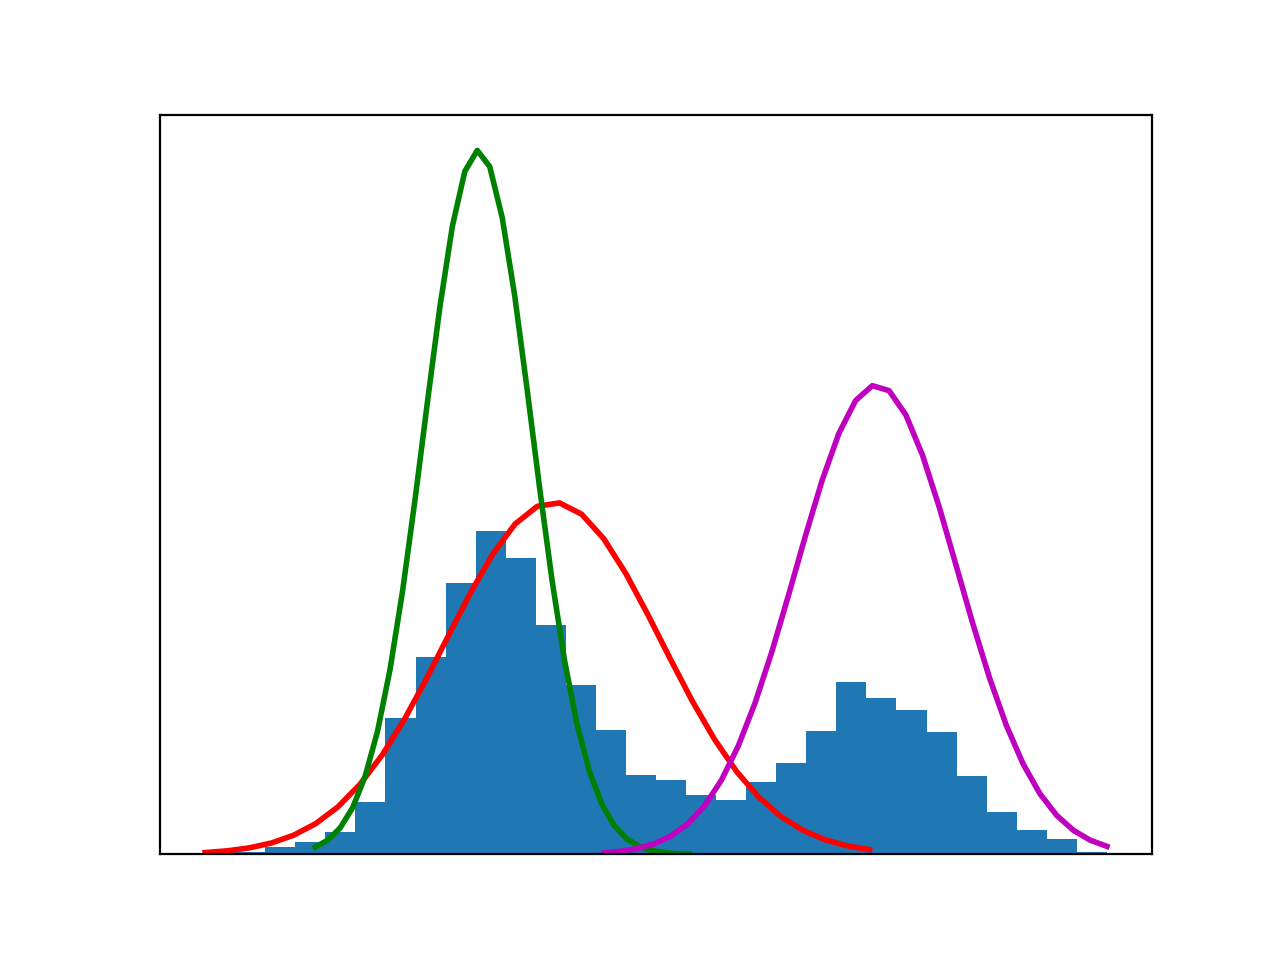
\includegraphics[width=1\textwidth]{lectEM/gmm.png}
\end{column}
\end{columns}
\end{frame}
%***********************************************************
\begin{frame}{Why Can't We Do Something Simple?}

\begin{columns}[T]
\begin{column}{0.5\textwidth}
\begin{itemize}
\item Like replace with the mean?
\begin{itemize}
	\item Back to the regression example
	\item Want a line to fit points $\langle 118, ?, 122, 145, 149, ?, 186 \rangle$
	\item Mean of observed data is 144
\end{itemize}
\end{itemize}
\end{column}
\begin{column}{0.5\textwidth}
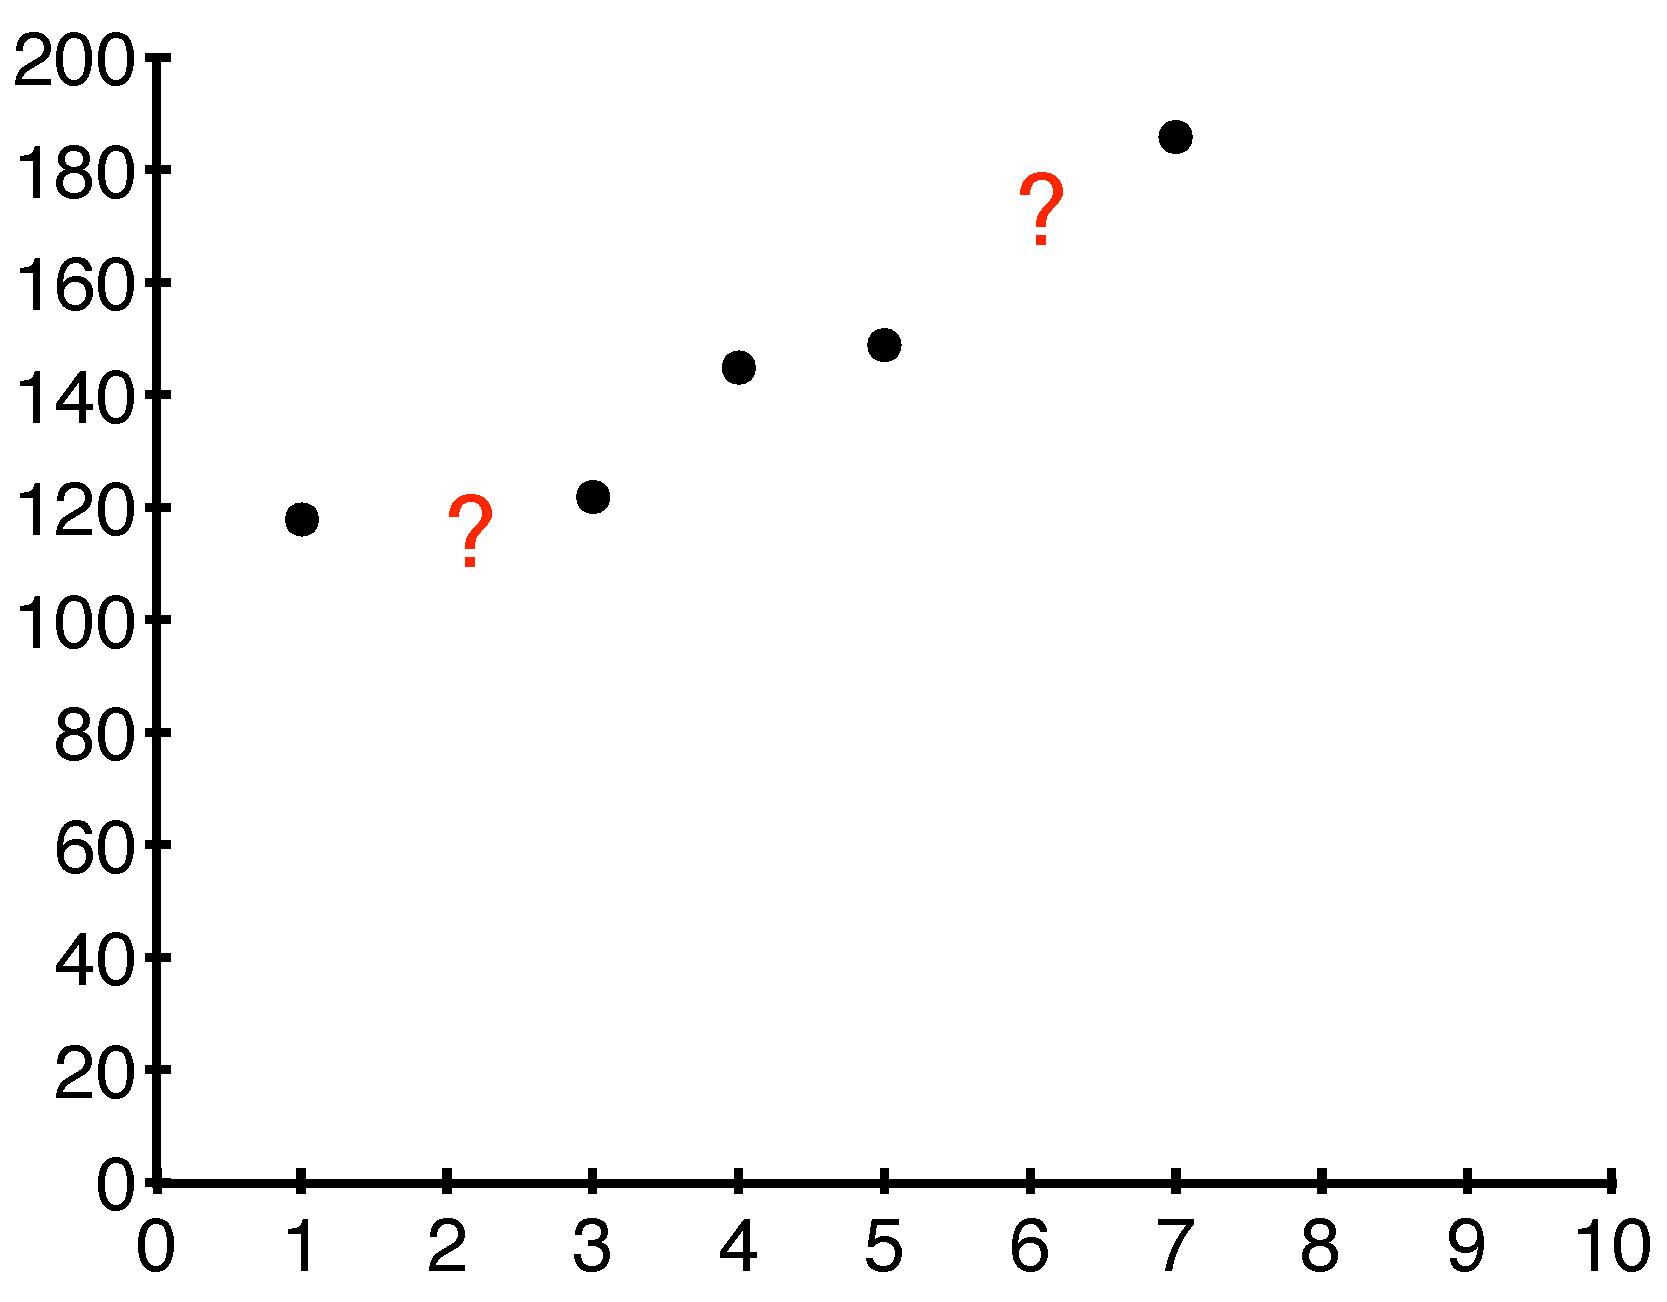
\includegraphics[width=1\textwidth]{lectEM/missingData1.pdf}
\end{column}
\end{columns}
\end{frame}
%***********************************************************
\begin{frame}{Why Can't We Do Something Simple?}

\begin{columns}[T]
\begin{column}{0.5\textwidth}
\begin{itemize}
\item Like replace with the mean?
\begin{itemize}
	\item Back to the regression example
	\item Want a line to fit points $\langle 118, ?, 122, 145, 149, ?, 186 \rangle$
	\item Mean of observed data is 144
	\item Does $\langle 118, 144, 122, 145, 149, 144, 186 \rangle$ make sense?
	\item No: given our regression model, we expect values in-keeping with model
\end{itemize}
\end{itemize}
\end{column}
\begin{column}{0.5\textwidth}
\includegraphics[width=1\textwidth]{lectEM/missingData1WithMean.pdf}
\end{column}
\end{columns}
\begin{itemize}
	\item EM lets us learn the model \& integrate over all possible values in a fancy way
\end{itemize}
\end{frame}
%***********************************************************
\begin{frame}{Can't We Just Drop the Data?}

\begin{itemize}
\item In our example, why not just learn from $\langle 118, 122, 145, 149, 186 \rangle$?
	\begin{itemize}
	\item Might make sense here...
	\item But not in general
	\item We can bias our data
	\item Or discard a lot of useful information if just one bit is missing
	\end{itemize}
\end{itemize}
\end{frame}
%***********************************************************
\begin{frame}{Hierarchical Models}

\begin{itemize}
\item In data science, often impossible to drop missing data
\item Because the data are missing (or hidden) by design
\item Happens with ``hierarchical models''
\end{itemize}
\end{frame}
%***********************************************************
\begin{frame}{Hierarchical Model Example}

\begin{columns}[T]
\begin{column}{0.5\textwidth}
	\begin{itemize}
		\item Have a bag with two coins 
		\item First has probability $p_1$ of heads
		\item Second has probability $p_2$ of heads
		\item I repeatedly reach in, pull out a coin
		\item Identity is $z_i \in \{1, 2\}$
		\item Flip it 10 times and observe $x_i$ heads
	\end{itemize}
\end{column}
\begin{column}{0.5\textwidth}
	\begin{itemize}
		\item 
		\item 
		\item 
		\item This is a trial over a RV
		\item Represents  coin selected at trial $i$
		\item Full dataset is $\{x_i, z_i\}$ pairs
	\end{itemize}
\end{column}
\end{columns}
\begin{itemize}
\item How do we compute $\Theta = \{p_1, p_2\}$?
\item Each $z_i$ is missing: we don't know identity of coin
\item[?] How could we just drop missing data in this case?  %we can't
\end{itemize}
\end{frame}
%***********************************************************
\begin{frame}{Formal Problem Definition}

\begin{itemize}
\item Formally: we want to compute an MLE for $L (\Theta | x_1, x_2, ..., z_1, z_2, ...)$
	\begin{itemize}
	\item $x_1, x_2, ...$ are observed data
	\item $z_1, z_2, ...$ are missing data
	\item $\Theta = \{p_1, p_2\}$, the probability of heads for each coin
	\end{itemize}
\item Recall
	\begin{itemize}
	\item This is just like computing the PDF
	\item The Likelihood function flips the parameters
	\item Measures how likely the parameters are given the data
	\end{itemize}

\end{itemize}


\end{frame}

%***********************************************************
\begin{frame}{Formal Problem Definition}

\begin{itemize}
\item Recall that:
	\begin{itemize}
	\item $L (\Theta | x_1, x_2, ..., z_1, z_2, ...) = f (x_1, x_2, ..., z_1, z_2, ... | \Theta)$
	\end{itemize}
\item When the $z$'s are missing, choose $\Theta$ to max 
	$$\int_{\langle z_1, z_2, ...\rangle} f (x_1, x_2, ..., z_1, z_2, ... | \Theta) d\langle z_1,z_2,...\rangle$$
\end{itemize}
\end{frame}


%***********************************************************
\begin{frame}{``Integrating out'' a Variable}

	$$\int_{\langle z_1, z_2, ...\rangle} f (x_1, x_2, ..., z_1, z_2, ... | \Theta) d\langle z_1,z_2,...\rangle$$
\begin{itemize}
\item Sum over all possible values of the variable you are integrating out
\item Example: say we have (height, weight) pairs
\item Probabilities are: $$\langle (\textrm{short}, \textrm{light}), 0.3 \rangle, 
	\langle (\textrm{short}, \textrm{heavy}), 0.1 \rangle, 
	\langle (\textrm{tall}, \textrm{light}), 0.2 \rangle, 
	\langle (\textrm{tall}, \textrm{heavy}), 0.4 \rangle$$
\item[] Probability they are ``tall'' is?
% note probabilities sum to 1
\end{itemize}
\end{frame}
%***********************************************************
\begin{frame}{``Integrating out'' a Variable}

	$$\int_{\langle z_1, z_2, ...\rangle} f (x_1, x_2, ..., z_1, z_2, ... | \Theta) d\langle z_1,z_2,...\rangle$$
\begin{itemize}
\item Sum over all possible values of the variable you are integrating out
\item Example: say we have (height, weight) pairs
\item Probabilities are: $$\langle (\textrm{short}, \textrm{light}), 0.3 \rangle, 
	\langle (\textrm{short}, \textrm{heavy}), 0.1 \rangle, 
	\langle (\textrm{tall}, \textrm{light}), 0.2 \rangle, 
	\langle (\textrm{tall}, \textrm{heavy}), 0.4 \rangle$$
\item Probability they are ``tall'' is $0.6 = \sum_{\textrm{weight } w} Pr[(\textrm{tall}, w)]$
\item Easy here, but difficult in the general case!
% In general, it's hard because of the integration.

\end{itemize}
\end{frame}

%***********************************************************
\begin{frame}{Expectation Maximization}

\begin{itemize}
\item Is an iterative algorithm for difficult missing-data MLEs
\item Basic idea...
	\begin{itemize}
	\item Have an estimate $\Theta^{\textrm{iter}}$ for each iteration
	\item Repeatedly update $\Theta^{\textrm{iter}}$ until convergence
	\item Looks a lot like gradient descent, right?
	\end{itemize}
\item But EM is unique in how it deals with missing data points
	\begin{itemize}
	\item The famous ``$Q$ function''
	$$Q(\Theta^{\textrm{iter}}, \Theta^{\textrm{iter }-1}) = E \left[ \log f (x_1, x_2, ..., z_1, z_2, ... | \Theta^{\textrm{iter}}) |
			x_1,  x_2, ..., \Theta^{\textrm{iter }-1} \right]$$
	\end{itemize}
\end{itemize}
\end{frame}
%***********************************************************
\begin{frame}{Expectation Maximization}

\begin{itemize}
\item How to interpret the $Q$ function?
	\begin{itemize}
	\item $Q$ function is:
	$$Q(\Theta^{\textrm{iter}}, \Theta^{\textrm{iter }-1}) = E \left[ \log f (x_1, x_2, ..., z_1, z_2, ... | \Theta^{\textrm{iter}}) |
			x_1,  x_2, ..., \Theta^{\textrm{iter }-1} \right]$$
	\item Treat $z_1, z_2, ...$ as random variables
	\item With distribution $f (z_1, z_2, ... | x_1,  x_2, ..., \Theta^{\textrm{iter }-1})$
	\item Kind of like Bayesian approach, with a prior and posterior distribution
	\item We're going to get something that looks like a posterior distribution over the $z$s
	\item The $Q$-function is the expected value of the LLH wrt this distribution
	\end{itemize}
\end{itemize}

\end{frame}
%***********************************************************
\begin{frame}{Expectation Maximization}

\begin{itemize}
\item What is expected value?
	\begin{itemize}
	\item Recall: expected value of $g(z)$ when $z$ has distribution (PDF) $f(z)$ is $\sum_z f(z) g(z)$ or $\int_z f(z) g(z) dz$
	\item When $z$ is discrete, $f(z)$ is a probability
	\item Example: If we sample $(A, B)$ from $$\langle (1, 2), .3 \rangle, 
		\langle (3, 5), 0.1 \rangle, 
		\langle (2, 6), 0.2 \rangle, 
		\langle (-3, 6), 0.4 \rangle$$
	\item $E[A + B] = 0.3 \times (1 + 2) + 0.1 \times (3 + 5) + 0.2 \times (2 + 6) + 0.4 \times (-3 + 6)$
	\end{itemize}
\end{itemize}
\end{frame}
%***********************************************************
\begin{frame}{Continuous and Discrete Q Function}

\begin{itemize}
	\item Continuous version is:
        $$Q(\Theta^{\textrm{iter}}, \Theta^{\textrm{iter }-1}) = E \left[ \log f (x_1, x_2, ..., z_1, z_2, ... | \Theta^{\textrm{iter}}) |
                        x_1,  x_2, ..., \Theta^{\textrm{iter }-1} \right]$$
	\item If $z$s are discrete (usually are):
		$$Q(\Theta^{\textrm{iter}}, \Theta^{\textrm{iter }-1}) =
			\sum_{\langle z_1, z_2, ... \rangle} f (z_1, z_2, ... | x_1,  x_2, ..., \Theta^{\textrm{iter }-1}) 
				\log f (x_1, x_2, ..., z_1, z_2, ... | \Theta^{\textrm{iter}})$$
%	\item where $f()$ is the density function
\end{itemize}
\end{frame}
%***********************************************************
\begin{frame}{What are the Values of Z?}

\begin{itemize}
\item The $z$s are often useful
\begin{itemize}
\item In a GMM, they tell you which cluster each data point belongs to
\end{itemize}
\item Running EM doesn't actually tell you the values of the $z$s
\item But, once you have $\Theta$ it's often easy to get the values
\item E.g. Use Bayes rule to find the posterior probability for each cluster
\end{itemize}
\end{frame}
%***********************************************************
\begin{frame}{Basic EM Algorithm}

\begin{itemize}
\item It is an iterative algorithm
	\begin{itemize}
	\item Start with a reasonable guess  for $\Theta$, call this $\Theta^0$
	\end{itemize}
\item In each iteration:
	\begin{itemize}
	\item Choose $\Theta^{\textrm{iter}}$ to maximize the expected value of the log-likelihood
	\end{itemize}
\item Stop when you can't improve any more
\end{itemize}
\end{frame}
%***********************************************************
\begin{frame}{Back to the Example}

\begin{itemize}
\item Best to return to our example...
	\begin{itemize}
	\item Bag with two coins
	\item $\Theta = \{p_1, p_2\}$: probability of each coin being heads
	\item $z_i \in \{1, 2\}$: identity of coin flip the $i$th time I reach in the bag
	\item $x_i \in \{0, ..., 10\}$: number of heads for the $i$th trial
	\end{itemize}
\item So where do we start?
\end{itemize}
\end{frame}
%***********************************************************
\begin{frame}{Back to the Example}

\begin{itemize}
\item Best to return to our example...
	\begin{itemize}
	\item Bag with two coins
	\item $\Theta = \{p_1, p_2\}$: probability of each coin being heads
	\item $z_i \in \{1, 2\}$: identity of coin flip the $i$th time I reach in the bag
	\item $x_i \in \{0, ..., 10\}$: number of heads for the $i$th trial
	\end{itemize}
\item So where do we start?
\item With the likelihood function!
\end{itemize}
\begin{columns}[T]
\begin{column}{0.5\textwidth}
	\begin{align}
	L (\Theta | x_1, x_2, ..., z_1, z_2, ...) &= f (x_1, x_2, ..., z_1, z_2, ... | \Theta) \nonumber \\
		&= \prod_i f (x_i, z_i | \Theta) \nonumber \\
		&= \prod_i \frac{1}{2} \textrm {Binomial}(x_i | p_{z_i}, 10) \nonumber
	\end{align}
\end{column}
\begin{column}{0.5\textwidth}
\begin{itemize}
\item Assume each action is independent % otherwise, don't use EM
\item $f()$ is the density function given our parameter set
\item $x_i$ is the $i$th \# of heads and $z_i$ is the identity of the $i$th coin selected
\end{itemize}
\end{column}
\end{columns}

		\end{frame}
%***********************************************************
\begin{frame}{Unpack the LLH Equation}

	\begin{align}
		&= \prod_i \frac{1}{2} \textrm {Binomial}(x_i | p_{z_i}, 10) \nonumber
	\end{align}
\begin{itemize}
\item $\frac{1}{2}$ is the 50/50 chance of pulling out each coin 
\item Binomial because it models coin flips 
\item 10 coin flips
\item $p_{z_i}$ = Probability of Heads for each $z_i$ (Recall: $z_i = \{1,2\}$)
\item We're using the identity of the coin to choose the right probability
\end{itemize}
\end{frame}
%***********************************************************
\begin{frame}{What About the Posterior for the Missing Data}

\begin{itemize}
\item Recall
		$$Q(\Theta^{\textrm{iter}}, \Theta^{\textrm{iter }-1}) =
			\sum_{\langle z_1, z_2, ... \rangle} f (z_1, z_2, ... | x_1,  x_2, ..., \Theta^{\textrm{iter }-1}) 
				\log f (x_1, x_2, ..., z_1, z_2, ... | \Theta^{\textrm{iter}})$$

\item Note $f (z_1, z_2, ... | x_1,  x_2, ..., \Theta^{\textrm{iter }-1}) = \prod_i f (z_i | x_i, \Theta^{\textrm{iter }-1})$
\item Can take product because we assume independence
	\begin{itemize}
	\item Use Bayes' rule!
	\end{itemize}
\begin{columns}[T]
\begin{column}{0.5\textwidth}
	\begin{align}
	f (z_i | x_i, \Theta^{\textrm{iter }-1}) &= 
		\frac{f (x_i, z_i | \Theta^{\textrm{iter }-1})}
		{f (x_i | \Theta^{\textrm{iter }-1})} \nonumber \\
	&= \frac{\frac{1}{2} \textrm {Binomial}(x_i | p_{z_i}^{\textrm{iter }-1}, 10)}
		{f (x_i | \Theta^{\textrm{iter }-1})} \nonumber
	\end{align}
\end{column}
\begin{column}{0.5\textwidth}
	\begin{itemize}
	\item Joint distribution of $x_i, z_i$ given the parameters
	\item Divided by a normalizing constant
	\end{itemize}
\end{column}
\end{columns}
	\item What is $f (x_i | \Theta^{\textrm{iter }-1})$?
	\end{itemize}
	
\end{frame}
%***********************************************************
\begin{frame}{Normalizing Constant}

\begin{itemize}
	\item What is $f (x_i | \Theta^{\textrm{iter }-1})$?
		$$f (x_i | \Theta^{\textrm{iter }-1}) = \frac{1}{2} \textrm {Binomial}(x_i | p_{1}^{\textrm{iter }-1}, 10) +
			\frac{1}{2} \textrm{Binomial}(x_i | p_{2}^{\textrm{iter }-1}, 10)$$
% coin 1 probability of the getting heads on a single trial + coin 2  probability of getting heads on a single trial 
	\item So, plug in these values to the equation on the previous slide to get:
		$$f (z_i | x_i, \Theta^{\textrm{iter }-1}) = \frac{\frac{1}{2} \textrm {Binomial}(x_i | p_{z_i}^{\textrm{iter }-1}, 10)}
			{\frac{1}{2} \textrm {Binomial}(x_i | p_{1}^{\textrm{iter }-1}, 10) +
                        \frac{1}{2} \textrm{Binomial}(x_i | p_{2}^{\textrm{iter }-1}, 10)}$$
        \item Cannot discard the denominator in this case, because with need the values to sum to 1 % because it's a PDF?
	\item Computing $f (z_i | x_i, \Theta^{\textrm{iter }-1})$ requires a pass over the data: called ``E-Step''
	\end{itemize}
\end{frame}
%***********************************************************
\begin{frame}{OK, got the E-Step, Now What?}

Now we need the M-Step, where we \textbf{maximize $Q$ wrt. $\Theta^{\textrm{iter}}$}
	\begin{itemize}
	\item Back to the $Q$ function:
		$$Q(\Theta^{\textrm{iter}}, \Theta^{\textrm{iter }-1}) =
			\sum_{\langle z_1, z_2, ... \rangle} f (z_1, z_2, ... | x_1,  x_2, ..., \Theta^{\textrm{iter }-1}) 
				\log f (x_1, x_2, ..., z_1, z_2, ... | \Theta^{\textrm{iter}})$$
	\item Let $c_{i, j}$ denote $f (z_i = j | x_i, \Theta^{\textrm{iter }-1})$
	$$Q(\Theta^{\textrm{iter}}, \Theta^{\textrm{iter }-1}) =\sum_{z_1} \sum_{z_2 } \sum_{z_3}... \left( \prod_i c_{i, z_i} \right) \log f (x_1, x_2, ..., z_1, z_2, ... | \Theta^{\textrm{iter}})$$
	\end{itemize}
\end{frame}
%***********************************************************
\begin{frame}{OK, got the E-Step, Now What?}

%	\begin{itemize}
%	\item Have $Q$ function:
		$$\sum_{z_1} \sum_{z_2 } \sum_{z_3}... \left( \prod_i c_{i, z_i} \right) \log f (x_1, x_2, ..., z_1, z_2, ... | \Theta^{\textrm{iter}})$$
	\begin{itemize}
	\item Where $\log f (x_1, x_2, ..., z_1, z_2, ... | \Theta^{\textrm{iter}})$ is:
	\end{itemize}
\begin{columns}[T]
\begin{column}{0.6\textwidth}
	\begin{align}
	\log \prod_i \textrm{Binomial} (x_i | p_{z_i}^{\textrm{iter }}) &=
		\sum_i \log \textrm{Binomial} (x_i | p_{z_i}^{\textrm{iter }}) \nonumber \\ &\propto
		\sum_i \log \left( 
			(p_{z_i}^{\textrm{iter }})^{x_i} \times (1 - p_{z_i}^{\textrm{iter }})^{10 - x_i} \right) \nonumber \\
			&=	\sum_i x_i \log (p_{z_i}^{\textrm{iter }}) + (10 - x_i) \log (1 - p_{z_i}^{\textrm{iter }}) \nonumber
	\end{align}
\end{column}
\begin{column}{0.4\textwidth}
{\footnotesize
	\begin{itemize}
	\item[]
	\item log of products = sum of logs
	\item Binomial PMF $\Big( {n \choose k } p^k(1-p)^{n-k}\Big)$has a combinatorial term, drop and switch to $\propto$
	\item Distribute the log function
	\end{itemize}
	}
\end{column}
\end{columns}
\end{frame}
%***********************************************************
\begin{frame}{OK, got the E-Step, Now What?}

	\begin{itemize}
	\item Dropping the ``iter'' on $p_{z_i}^{\textrm{iter }}$ (since both terms have it), the $Q$ function becomes:
	\begin{align}
		\sum_{z_1} \sum_{z_2 } \sum_{z_3}... \left( \prod_i c_{i, z_i} \right) \sum_i x_i \log (p_{z_i}) + (10 - x_i) \log (1 - p_{z_i}) \nonumber
	\end{align}
	\item Note: We are summing over an exponential number of items
	\end{itemize}\end{frame}
%***********************************************************
\begin{frame}{The M-Step}

	\begin{itemize}
	\item Now, we need to maximize:
		$$\sum_{z_1} \sum_{z_2 } \sum_{z_3}... \left( \prod_i c_{i, z_i} \right) \sum_i x_i \log (p_{z_i}) + (10 - x_i) \log (1 - p_{z_i})$$
	\item Ugly!  Or is it?  Consider just one variable, $z_1$.  Write as:
		\begin{align}
		&\sum_{z_1} \sum_{\langle z_2, z_3, ... \rangle} c_{1, z_1} a(\langle z_2, z_3, ... \rangle) 
	           \left(x_1 \log (p_{z_1}) + (10 - x_1) \log (1 - p_{z_1}) + \sum_{i = 2}^n b (\langle z_2, z_3, ... \rangle) \right) \nonumber \\
		&= \sum_{\langle z_2, z_3, ... \rangle} c_{1, 1} a(\langle z_2, z_3, ... \rangle) 
			\left(x_1 \log (p_1) + (10 - x_1) \log (1 - p_1) + \sum_{i = 2}^n b (\langle z_2, z_3, ... \rangle) \right) 
\nonumber \\ % coin 1
		&+ \sum_{\langle z_2, z_3, ... \rangle} c_{1, 2} a(\langle z_2, z_3, ... \rangle) 
			\left(x_1\log (p_2) + (10 - x_1) \log (1 - p_2) + \sum_{i = 2}^n b (\langle z_2, z_3, ... \rangle) \right)  % coin 2
\nonumber
		\end{align}
		\item where $a$ is the terms in $\prod_i c_{i, z_i}$ except for the current coin flip
		\item where $b$ is the terms in the sum over the $x_i$ except for the current coin flip
	\end{itemize}
\end{frame}
%***********************************************************
\begin{frame}{The M-Step}

{\footnotesize
		\begin{align}
		&c_{1, 1} \sum_{\langle z_2, z_3, ... \rangle} a(\langle z_2, z_3, ... \rangle) 
			\left(x_1\log (p_1) + (10 - x_1) \log (1 - p_1) + \sum_{i = 2}^n b (\langle z_2, z_3, ... \rangle) \right) 
\nonumber \\
		&+ c_{1, 2} \sum_{\langle z_2, z_3, ... \rangle} a(\langle z_2, z_3, ... \rangle) 
			\left(x_1\log (p_2) + (10 - x_1) \log (1 - p_2) + \sum_{i = 2}^n b (\langle z_2, z_3, ... \rangle) \right) 
\nonumber 
		\end{align}
	\begin{itemize}
	\item Continuing, split into the actual two terms, one for each coin, then distribute the $c$ terms:
		\begin{align}
		&= c_{1, 1} \left(x_1\log (p_1) + (10 - x_1) \log (1 - p_1) \right) \sum_{\langle z_2, z_3, ... \rangle} a(\langle z_2, z_3, ... \rangle) 
\nonumber \\
		&+ c_{1, 1} \sum_{\langle z_2, z_3, ... \rangle} a(\langle z_2, z_3, ... \rangle) \sum_{i = 2}^n b (\langle z_2, z_3, ... \rangle)  
\nonumber \\
		&+ c_{1, 2} \left(x_1\log (p_2) + (10 - x_1) \log (1 - p_2) \right) \sum_{\langle z_2, z_3, ... \rangle} a(\langle z_2, z_3, ... \rangle) 
\nonumber \\
		&+ c_{1, 2} \sum_{\langle z_2, z_3, ... \rangle} a(\langle z_2, z_3, ... \rangle) \sum_{i = 2}^n b (\langle z_2, z_3, ... \rangle)  
\nonumber 
		\end{align}
	\end{itemize}
	}
	\end{frame}
%***********************************************************
\begin{frame}{The M-Step}

	\begin{itemize}
	\item Continuing, recombine in a simpler way \& drop the  $\sum_{\langle z_2, z_3, ... \rangle} a(\langle z_2, z_3, ... \rangle)$ from the first term:
		\begin{align}
		&c_{1, 1} \left(x_1\log (p_1) + (10 - x_1) \log (1 - p_1) \right) \sum_{\langle z_2, z_3, ... \rangle} a(\langle z_2, z_3, ... \rangle) 
\nonumber \\
		&+ c_{1, 1} \sum_{\langle z_2, z_3, ... \rangle} a(\langle z_2, z_3, ... \rangle) \sum_{i = 2}^n b (\langle z_2, z_3, ... \rangle)  
\nonumber \\
		&+ c_{1, 2} \left(x_1\log (p_2) + (10 - x_1) \log (1 - p_2) \right) \sum_{\langle z_2, z_3, ... \rangle} a(\langle z_2, z_3, ... \rangle) 
\nonumber \\
		&+ c_{1, 2} \sum_{\langle z_2, z_3, ... \rangle} a(\langle z_2, z_3, ... \rangle) \sum_{i = 2}^n b (\langle z_2, z_3, ... \rangle)  
\nonumber \\
		&= c_{1, 1} \left(x_1\log (p_1) + (10 - x_1) \log (1 - p_1) \right) + \nonumber \\ 
		&+ c_{1, 2} \left(x_1\log (p_2) + (10 - x_1) \log (1 - p_2) \right) + \nonumber \\
		&+ \sum_{\langle z_2, z_3, ... \rangle} a(\langle z_2, z_3, ... \rangle) \sum_{i = 2}^n b (\langle z_2, z_3, ... \rangle) \nonumber
		\end{align}
	\end{itemize}
\end{frame}
%***********************************************************
\begin{frame}{The M-Step}

	\begin{itemize}
	\item Question: why can we drop $\sum_{\langle z_2, z_3, ... \rangle} a(\langle z_2, z_3, ... \rangle)$ from:
	\begin{align}
	c_{1, 1} \left(x_1\log (p_1) + (10 - x_1) \log (1 - p_1) \right) \sum_{\langle z_2, z_3, ... \rangle} a(\langle z_2, z_3, ... \rangle) \nonumber
	\end{align}
	\item Answer: $a(\langle z_2, z_3, ... \rangle)$ is the posterior probability of flip sequence 2 coming from coin $z_2$ and flip sequence 3 coming from coin $z_3$ and
	flip sequence 4 coming from coin $z_4$ and so on.
	\item Since we sum over all possible $\langle z_2, z_3, ... \rangle$, we are summing the probability all possible identities for coins $2, 3, 4...$
	\item This has to equal 1!  
	\item Why? By definition, when you sum the probability of all possibilities, you get 1
	\end{itemize}
	\end{frame}
%***********************************************************
\begin{frame}{The M-Step}
	\begin{itemize}
	\item Note the last term in
		\begin{align}
		c_{1, 1} \left(x_1\log (p_1) + (10 - x_1) \log (1 - p_1) \right) + \nonumber \\ 
		+ c_{1, 2} \left(x_1\log (p_2) + (10 - x_1) \log (1 - p_2) \right) + \nonumber \\
		+ \sum_{\langle z_2, z_3, ... \rangle} a(\langle z_2, z_3, ... \rangle) \sum_{i = 2}^n b (\langle z_2, z_3, ... \rangle) \nonumber
		\end{align}
	\item This is like a ``littler'' $Q$-function, or what we get after removing the first coin flip ($z_1$). So we have shown the $Q$-function is just:
		\begin{align}
		c_{1, 1} \left(x_1\log (p_1) + (10 - x_1) \log (1 - p_1) \right) + \nonumber \\
		c_{1, 2} \left(x_1\log (p_2) + (10 - x_1) \log (1 - p_2) \right) + \nonumber \\
		\sum_{z_2 } \sum_{z_3}... \left( \prod_{i \geq 2} c_{i, z_i} \right) \sum_{i \geq 2} x_i \log (p_{z_i}) + (10 - x_i) \log (1 - p_{z_i}) \nonumber
		\end{align}
	\end{itemize}
\end{frame}
%***********************************************************
\begin{frame}{The M-Step}
        \begin{itemize}
	\item So we've shown we can remove $z_1$ from the nasty summation $\sum_{z_1} \sum_{z_2 } \sum_{z_3}...$
	\item We can use the same algebraic manipulations to get rid of $z_2$, then $z_3$, etc., giving us:
		$$\sum_i c_{i, 1} \left(x_i\log (p_1) + (10 - x_i) \log (1 - p_1) \right) 
			+ c_{i, 2} \left(x_i\log (p_2) + (10 - x_i) \log (1 - p_2) \right)$$
	\end{itemize}
\end{frame}
%***********************************************************
\begin{frame}{The M-Step}

{\small
	\begin{itemize}
	\item Now we maximize wrt $p_1$, $p_2$
	\item Partial derivative wrt $p_1$:
		$$\sum_i c_{i, 1} x_i \frac{1}{p_1} - \sum_i c_{i, 1} (10 - x_i) \frac{1}{1 - p_1}$$
	\item Set to zero:
	\begin{align}
		\sum_i c_{i, 1} x_i \frac{1}{p_1} - \sum_i c_{i, 1} (10 - x_i) \frac{1}{1 - p_1} = 0 \nonumber \\
		\frac{1}{p_1} \sum_i c_{i, 1} x_i - \frac{1}{1 - p_1} \sum_i 10 c_{i, 1} + \frac{1}{1 - p_1} \sum_i c_{i, 1} x_i = 0 \nonumber \\
		(1 - p_1) \sum_i c_{i, 1} x_i - p_1 \sum_i 10 c_{i, 1} + p_1 \sum_i c_{i, 1} x_i = 0 \nonumber \\
		\sum_i c_{i, 1} x_i - p_1 \sum_i 10 c_{i, 1} = 0 \nonumber \\
		p_1 = \frac{\sum_i c_{i, 1} x_i}{\sum_i 10 c_{i, 1}} \nonumber
	\end{align}
	\end{itemize}
	}
  	\end{frame}
%***********************************************************
\begin{frame}{The M-Step}

	\begin{itemize}
	\item Recall: $c_{i, j}$ denotes $f (z_i = j | x_i, \Theta^{\textrm{iter }-1})$
	\item Let's consider
		$$p_1 = \frac{\sum_i c_{i, 1} x_i}{\sum_i 10 c_{i, 1}} $$
	\item We are taking a weighted sum that looks at how many times, out of 10, we got heads
	\item Taking into account a weighting factor  that each data point was effected by $c_1$ %(the posterior probability)
	\item We can repeat for $c_2$
	\end{itemize}
  	\end{frame}
%***********************************************************
\begin{frame}[fragile]{The M-Step}
        \begin{itemize}
	\item So, $p_2 = \frac{\sum_i c_{i, 2} x_i}{\sum_i 10 c_{i, 2}}$
	\item Very simple!!
	\end{itemize}
\begin{SQL}
set $p_1$ = 0.8, $p_2$ = 0.2
while ($p_1$, $p_2$ still change) do
  compute $c_{i, 1}$, $c_{i, 2}$ for each $i$
  set $p_1$ = $\frac{\sum_i c_{i, 1} x_i}{\sum_i 10 c_{i, 1}}$
  set $p_2$ = $\frac{\sum_i c_{i, 2} x_i}{\sum_i 10 c_{i, 2}}$
end while 
\end{SQL}
        \begin{itemize}
	\item But a long way to get there 
	\end{itemize}
\end{frame}

%***********************************************************
\begin{frame}[fragile]{A Quick Review}
        \begin{itemize}
	\item Goal: Find the model parameters, $p_1$ and $p_2$
	\item Given: Observations of the number of heads in 10 coin tosses, over a number of trials	
	\item It's (relatively) easy if we know which coin was selected during each trial
	$$p_1 = \frac{\textrm{\# of heads using coin 1}}{\textrm{total \# of flips using coin 1}}$$
	$$p_2 = \frac{\textrm{\# of heads using coin 2}}{\textrm{total \# of flips using coin 2}}$$
	\end{itemize}
\end{frame}

%***********************************************************
\begin{frame}[fragile]{A Quick Review}
        \begin{itemize}
	\item If we don't know which coin was selected for each trial, we need to estimate it
	\item We could do this by
	        \begin{enumerate}
		\item Computing the most likely coin selected for each observation, given an estimate of $p_1$ and $p_2$
		\item Then use these assignments to compute a revised MLE estimate of the parameters
		\item Repeat until $p_1$ and $p_2$ converge
		\end{enumerate}
	\end{itemize}
\end{frame}
%***********************************************************
\begin{frame}[fragile]{A Quick Review}
        \begin{itemize}
	\item Alternatively, we could 
	        \begin{itemize}
		\item Compute the probability for each possible combination of the selected coins
		\item Use these probabilities to build a weighted function of the data to determine the probabilities
		\item And re-estimate the parameters, using the weighted functions in an MLE
		\vspace{1 em}
		\item Alternate between guessing the distribution of the missing data (the E-step)
		\item And re-estimating the parameter values (the M-step)
		\end{itemize}
	\end{itemize}
\end{frame}
%***********************************************************
\begin{frame}{Thoughts about EM}
\begin{itemize}
\item EM requires a lot of thinking and a lot of math
\item It's very efficient (great for big data)
\item However, if you have a lot of missing data
\begin{itemize}
\item Use Markov Chain Monte Carlo (MCMC) / Bayesian methods 
\item Easier than EM
\item Not as efficient
\end{itemize}
\end{itemize}
\end{frame}
%***********************************************************
\begin{frame}{Questions?}
\begin{itemize}
	\item What do we know now that we didn't know before?

	\item How can we use what we learned today?
\end{itemize}
\end{frame}


\end{document}
